% Beyond Marginal Coverage -- 3ICT 2026, revised after conditional acceptance.
%
% Build:  latexmk -pdf main.tex
%
% Every numeral traces to a CSV in ../results/metrics/. `python claims.py`
% recomputes the headline numbers and requires each to be printed here;
% `python verify.py` checks citations, graphics, cross-references and float
% order.
%
% a4paper: 3ICT distributes "Conference-template-A4.doc" as its Word template,
% not IEEE's generic US-letter one, so A4 is this venue's own choice.
\documentclass[a4paper,conference]{IEEEtran}
\IEEEoverridecommandlockouts

\usepackage{cite}
\usepackage{amsmath,amssymb}
\usepackage{graphicx}
\usepackage{booktabs}
\usepackage{tikz}
\usepackage{url}
\usepackage[hidelinks]{hyperref}

\graphicspath{{figures/}}

\newcommand{\Dtrain}{\mathcal{D}_{\mathrm{train}}}
\newcommand{\Dthr}{\mathcal{D}_{\mathrm{thr}}}
\newcommand{\Dcal}{\mathcal{D}_{\mathrm{cal}}}
\newcommand{\Dtest}{\mathcal{D}_{\mathrm{test}}}
\newcommand{\sbase}{s_{\mathrm{base}}}
% Reviewer-comment tags: empty here, printed in the highlighted build.
\newcommand{\rtag}[1]{}

\begin{document}

\title{Beyond Marginal Coverage: Auditing Conformal\\
Prediction for Medical VQA}

\author{\IEEEauthorblockN{Ahmed Mellit\IEEEauthorrefmark{1}\thanks{Corresponding
author: Ahmed Mellit (ahmed\_mellit@um5.ac.ma).},
Achraf Cohen\IEEEauthorrefmark{2},
Hafssa Benaboud\IEEEauthorrefmark{1}}
\IEEEauthorblockA{\IEEEauthorrefmark{1}IPSS Laboratory, Faculty of Sciences,
Mohammed V University, Rabat, Morocco}
\IEEEauthorblockA{\IEEEauthorrefmark{2}Department of Mathematics and Statistics,
University of West Florida, Pensacola, FL, USA}}

\maketitle

\begin{abstract}
Conformal prediction can turn a frozen medical vision--language model into a
set-valued predictor with a finite-sample marginal coverage guarantee. We ask
what that guarantee leaves unexamined, varying the protocol around three
post-hoc scores (LAC, APS and RAPS) over 20 re-splits of OmniMedVQA and
VQA-RAD with cached outputs of Qwen2.5-VL-3B and, as a second backbone,
Qwen3-VL-4B.\rtag{R1.1} On the balanced OmniMedVQA sample, a head that sees
only answer-string embeddings reaches $95.3\%$ top-1 accuracy, so high accuracy
and small sets there are weak evidence of visual reasoning. Tuning
hyperparameters on the calibration set lowers coverage by up to $1.3$
percentage points, significantly on some model--corpus pairs and not others.
On binary VQA-RAD, temperature-only LAC produces the same conformal sets at
every temperature up to floating-point ties, whereas APS without its internal
randomization returns both options for every question on both backbones,
because a third or more of its calibration scores sit at the score's
maximum.\rtag{R2.1} On Qwen2.5-VL-3B, near-nominal marginal coverage hides an
ultrasound coverage of $0.709$, a letter-dependent profile across cyclic option
orders and, on VQA-RAD, lower coverage of questions whose answer is ``no''; on
Qwen3-VL-4B the undercovered modality changes and the answer gap reverses.
Worst-group comparisons across partitions must account for group sizes. The
findings concern the evaluated models and corpora, and coverage under
stratified and image-disjoint splits is empirical rather than
guaranteed.\rtag{R2.6}
\end{abstract}

\begin{IEEEkeywords}
conformal prediction, uncertainty quantification, medical visual question
answering, conditional coverage, benchmarking, evaluation protocol
\end{IEEEkeywords}

\section{Introduction}\label{sec:intro}

A medical vision--language model (VLM) answering a multiple-choice question
returns an option and a confidence that is generally not calibrated
\cite{guo2017calibration}. Conformal prediction wraps such a model in a
set-valued predictor whose sets contain the truth with a chosen probability, in
finite samples, under exchangeability, with no retraining
\cite{vovk2005algorithmic,lei2018distribution,angelopoulos2023gentle}. The
guarantee is marginal: it holds on average over the population, and
distribution-free coverage at almost every input is unattainable for
non-trivial sets \cite{foygelbarber2021limits}. It also presumes a protocol in
which the score is fixed before the calibration labels are read.

\textbf{Positioning.} Azad et al.\ \cite{azad2026maybe} benchmark conformal
prediction across 18 VLMs with the protocol held fixed; we hold the model fixed
and vary the protocol. Medical work improves the score, by transductive
adaptation on the joint calibration and test pool
\cite{silvarodriguez2025sca,bozorgtabar2026lata} or by conformal transfer of
frozen VLMs \cite{silvarodriguez2025zeroshot,silvarodriguez2025fca}. A better
score does not remove the need to audit how the calibration data are split,
searched and presented, although some of the effects below depend on the
score's distribution. Zeng et al.\ \cite{zeng2025tuningbias} analyse the
coverage cost of tuning on the calibration set, and Liang et al.\
\cite{liang2024selection} construct valid sets after data-dependent selection;
we measure that cost in a medical VQA pipeline.

\textbf{Claim and contributions.} On two selected medical VQA corpora and two
frozen backbones, benchmark shortcuts and calibration or presentation choices
materially change how conformal coverage and efficiency should be read, and
marginal coverage with mean set size misses these effects. The evidence answers
three questions. \emph{What does the benchmark reward?} Answer-only and
question-only controls (Section~\ref{sec:shortcut}). \emph{Which protocol
choices change the conformal predictor?} Calibration reuse and APS
randomization (Section~\ref{sec:protocol}). \emph{What does marginal coverage
conceal?} Subgroup gaps read against a reference, and option-order analyses on
both corpora (Section~\ref{sec:beyond}). Section~\ref{sec:backbone} repeats the
protocol analyses on a second backbone, and Section~\ref{sec:discussion}
separates what is expected to hold generally from what is specific to these
models and corpora.

\section{Setup and validity scope}\label{sec:setup}

\textbf{Data.} \emph{OmniMedVQA} \cite{hu2024omnimedvqa}, open-access split:
3{,}000 items drawn $375$ per imaging modality across eight modalities, so the
marginal target is that balanced mixture, not natural prevalence. Option counts
are mixed ($2{,}745$ at $K{=}4$, $248$ at $K{=}2$, $7$ at $K{=}3$; mean
$K=3.83$), on 2{,}990 distinct images. \emph{VQA-RAD} \cite{lau2018vqarad},
closed yes/no subset: 1{,}191 questions on 294 images, $49.1\%$ ``yes''. The
copy we read has no organ field, so each image's organ comes from the original
release's \texttt{image\_organ} field, matched on the image's set of questions.
$290$ images match exactly one released image; the other four form two pairs,
each sharing a single question with two released images, one pair whose
candidates have the same organ and one resolved by inspecting the images. This
gives head ($308$ questions), chest ($475$) and abdomen ($408$).\rtag{C1}

\textbf{Models and scores.} A frozen \texttt{Qwen2.5-VL-3B-Instruct}
\cite{bai2025qwen25vl} is run once per item under the letter-logit protocol of
medical VQA leaderboards \cite{lai2025medr1}: image, question, options as lines
``A.~\ldots'' onward, and an instruction to answer with the letter. A
full-vocabulary log-softmax at the first generated position gives
$\sbase(x,y_k)=-\log p(\text{letter}_k\mid x)$. The second backbone,
\texttt{Qwen3-VL-4B-Instruct} \cite{bai2025qwen3vl}, a later generation at a
larger scale, is run in bfloat16, its native precision, and scored with the
same prompt and the same rule.\rtag{R1.1} Scores are cached, so every method
sees byte-identical inputs.

\textbf{Splits and roles.} Each re-split draws a partition
$\Dtrain\cup\Dthr\cup\Dcal\cup\Dtest$ in proportions $0.50/0.15/0.15/0.20$,
stratified on modality or organ. VQA-RAD asks $4.05$ questions per image, and
an item-level split leaves $94.7\%$ of test questions with their image in
another partition, so VQA-RAD is split by image: whole images are shuffled
within stratum and placed greedily against item quotas (realized test share
$0.200$). OmniMedVQA stays item-level; there only $0.5\%$ of test items share
an image across partitions. Hyperparameters are chosen on $\Dthr$ alone, halved
so a provisional threshold is fitted on one half and mean set size measured on
the other (Fig.~\ref{fig:roles}); $\Dcal$ is read once, for the final
threshold. The grids are temperatures $T\in\{0.25,0.5,1,2,4,8\}$ for all three
scores and, for RAPS, $\gamma\in\{0,0.01,0.05,0.1,0.3\}\times
k_{\mathrm{reg}}\in\{1,2\}$, $60$ configurations, searched with $T$ outermost
and the first configuration kept on ties.\rtag{R2.2}

\textbf{Scores.} With $\hat p(y|x)$ the temperature-scaled softmax of
$-\sbase$, \textbf{LAC} uses $s=1-\hat p(y|x)$ \cite{sadinle2019least};
\textbf{APS} uses $s=\sum_{j<\mathrm{rank}(y)}\hat p_{(j)}(x)+u\,\hat p_y(x)$
with a uniform $u$ \cite{romano2020classification}, and $u=1$ is its
deterministic variant; \textbf{RAPS} adds
$\gamma\max(0,\mathrm{rank}-k_{\mathrm{reg}})$ \cite{angelopoulos2021uncertainty}.
Ranks sort $\hat p$ stably, so equal probabilities are ordered by option index.

\textbf{Randomness and thresholds.} APS and RAPS take one uniform per
candidate from a keyed hash of (re-split, item, option). Distinct items never
share a draw.\rtag{C2} An item's option keeps its draw under every configuration, arm,
calibration subset and cyclic rotation, which pairs those comparisons, and APS
and RAPS share draws. The re-split index also seeds the partition and the
halving of $\Dthr$. The threshold is the order statistic itself: with $n$
calibration scores and $k=\lceil(n+1)(1-\alpha)\rceil$, $\tau$ is the $k$-th
smallest ($\tau=\infty$ if $k>n$), ties are kept and no noise is added.\rtag{C3}
Restarting one generator at every scoring call instead, which gives calibration
row $j$ and test row $j$ the same draws, changes mean Table~\ref{tab:main}
coverage by at most $0.0025$ (all paired $p\ge0.42$).

\textbf{Guarantee.} The set $C(x)=\{y:s(x,y)\le\tau\}$ satisfies
$\Pr[Y\in C(X)]\ge1-\alpha$ when calibration and test scores, auxiliary draws
included, are exchangeable \cite{vovk2005algorithmic,lei2018distribution}, and
coverage is at most $1-\alpha+1/(n+1)$ if the scores are also almost surely
distinct. Empty sets take the \texttt{argmax} option. Coverage and size are
reported after this fallback and empty rates before it; the fallback only
enlarges sets, so it cannot lower coverage but voids the upper bound. Mondrian
calibration fits one $\tau_g$ per level of a partition known at inference
\cite{vovk2003mondrian}, finite only if $n_g\ge\lceil(1-\alpha)/\alpha\rceil$,
which is $9$ at $\alpha=0.10$ \cite{ding2023class}.

\textbf{Validity scope.} Our partitions are stratified with fixed quotas, and
VQA-RAD assigns whole images while calibrating and scoring per question. Image
disjointness removes shared images across partitions; it does not make
questions about one image independent. Neither design is a uniform random
partition of exchangeable units, so all coverage we report is an empirical
property of these protocols, not an instance of the theorem; hierarchical
conformal prediction \cite{dunn2023hierarchical} targets image-level
guarantees. An interval containing $0.90$ establishes neither validity nor
equality to nominal.\rtag{R2.6}

\textbf{Statistics.} The 20 re-splits resample one fixed corpus, so inference
concerns the mean over this splitting procedure conditional on the corpus, not
new datasets or patients. Intervals are
$\bar x\pm t_{0.975,19}\,s/\sqrt{20}$, uncertainty in that mean, which is
narrower than the spread of single-split outcomes.\rtag{R2.4} Paired comparisons use the
paired $t$-test; significance statements and table stars use its
Holm-adjusted $p$ \cite{holm1979simple}, and the Wilcoxon signed-rank $p$
\cite{wilcoxon1945individual} beside it is raw. Two confirmatory families are
corrected over the three scores, separately per dataset: \emph{leakage},
coverage under the leaky-full arm against the clean arm at each score's full
grid (Section~\ref{sec:protocol}), where LAC's identically zero contrast on
VQA-RAD enters with $p=1$; and \emph{ensembling}, the per-split position spread
under the order ensemble against the original order (Section~\ref{sec:order}).
All other tests are exploratory and corrected, where at all, within the family
named beside them.

\section{What the benchmark rewards}\label{sec:shortcut}

Before comparing scores we ask what OmniMedVQA rewards. A head scores option
$y$ as $s(x,y)=\sbase(x,y)+g([z_x;e_y])$, with $z_x$ the pooled final hidden
state, $e_y$ the option embedding and $g$ an MLP
($2\,048{+}2\,048\to256\to128\to1$; Adam at $10^{-3}$, weight decay $10^{-4}$,
batch 64, early-stopped on $\Dthr$ top-1), trained on the cached features by
cross-entropy. The \emph{answer-only} variant zeroes $z_x$ and $\sbase$,
leaving $g([0;e_y])$. The embedding $e_y$ is the frozen model's input-embedding
table applied to that option string alone and mean-pooled: it passes through no
transformer layer and sees no image, question or other option, and letter and
order are not inputs. Both heads are trained separately on every re-split with
the same architecture, optimizer, batch size, seed and stopping rule; only the
zeroed inputs differ.\rtag{R2.3}

On OmniMedVQA the answer-only head reaches top-1 $0.953$, against $0.955$ with
every feature, a paired difference of $-0.0025$ [$-0.0058$, $+0.0008$];\rtag{R2.3} the
frozen base
score reaches $0.663$ and uniform guessing $0.271$. A lookup with no model at
all scores each option string $a$ by
\begin{equation*}
\hat q(a)=\frac{\#\{\text{training occurrences of }a\text{ as the correct option}\}}
{\#\{\text{training occurrences of }a\text{ among the options}\}},
\end{equation*}
gives strings unseen in training the pooled rate, breaks ties uniformly at
random and picks the highest-scoring option; it reaches $0.916$. The $3{,}000$
items draw on $1{,}244$ distinct option strings, and $97.4\%$ of test answers
occur among training options. On the rest, about $15$ items per split, pooled
as item--split occurrences (a question can recur across re-splits), the lookup
falls to $0.474$ while the answer-only head keeps $0.649$; the lookup does not
capture everything the head exploits, which may, for instance, rule out
distractor strings it has seen. The shortcut is broad: the answer-only head's
top-1 runs from $0.906$ (X-ray) to $0.990$ (OCT) across the eight modalities.
On ultrasound it reaches $0.973$ where the lookup gets $0.747$ and the frozen
model $0.405$. String-associated
answer priors explain a substantial part of the control's performance, but the
experiment does not identify its mechanism uniquely.\rtag{R2.3}

VQA-RAD needs a different control, since its options are always yes/no: the
answer-only head reaches $0.480$ and the answer lookup $0.476$, chance. Its
questions do recur across images, though, so we also look up each normalized
question string's majority answer in training. That reaches $0.507$, because
only $15.4\%$ of test questions occur in training; on those the lookup gets
$0.695$ against $0.632$ for the frozen model. A question prior exists, on a
small share of the corpus.\rtag{R1.6}

The consequence is a scope limit, not a finding about test-label access or a
flaw in coverage arithmetic. On this OmniMedVQA sample, high accuracy and
near-singleton sets from a learned score cannot be attributed to visual
reasoning from these data alone, so the rest of the paper studies post-hoc
scores over the frozen models' output.\rtag{R1.W}

\section{Calibration protocol effects}\label{sec:protocol}

\begin{table}[tb]
\caption{Post-hoc scores at $\alpha=0.10$ on Qwen2.5-VL-3B, means over 20
re-splits with $95\%$ intervals for coverage. \emph{Worst}: each split's lowest
per-modality (OmniMedVQA) or per-organ (VQA-RAD) coverage, averaged.}
\label{tab:main}
\centering
\footnotesize
\begin{tabular}{lllr}
\toprule
Score & Coverage [95\% CI] & Size & Worst \\
\midrule
\multicolumn{4}{l}{\emph{OmniMedVQA} (top-1 $0.663$)}\\
LAC  & 0.903 [0.896, 0.911] & 1.752 & 0.709 \\
APS  & 0.904 [0.895, 0.913] & 1.832 & 0.753 \\
RAPS & 0.903 [0.898, 0.909] & 1.839 & 0.725 \\
\midrule
\multicolumn{4}{l}{\emph{VQA-RAD} (image-disjoint, top-1 $0.654$)}\\
LAC  & 0.907 [0.891, 0.923] & 1.572 & 0.868 \\
APS  & 0.911 [0.896, 0.926] & 1.626 & 0.880 \\
RAPS & 0.908 [0.893, 0.923] & 1.617 & 0.881 \\
\bottomrule
\end{tabular}
\end{table}

Under the standard protocol the three scores are close (Table~\ref{tab:main}):
mean coverage lies between $0.903$ and $0.911$, the largest set-size gap is
$0.087$ options, on OmniMedVQA, and pre-fallback empty rates are at most
$0.005$. Protocol choices move them further; Table~\ref{tab:effects} collects
every protocol contrast in the paper, with its interval and corrected $p$.\rtag{R1.5, R2.4}

\begin{table*}[tb]
\caption{Protocol effects on Qwen2.5-VL-3B: paired changes over 20 re-splits,
intervention minus reference, with $95\%$ intervals. \emph{Reuse, full}:
leaky-full minus clean; \emph{reuse, matched}: leaky minus clean
(Fig.~\ref{fig:roles}); \emph{no randomization}: APS with $u=1$ minus APS;
\emph{order ensemble}: averaged over cyclic orders minus the original order,
where the coverage column is the per-split position spread; \emph{image split}:
image-disjoint minus item-level. $p$ is Holm-adjusted within the contrast's
family (Section~\ref{sec:setup}).}
\label{tab:effects}
\centering
\footnotesize
\begin{tabular}{llllll}
\toprule
Intervention & Data & Score & $\Delta$ coverage [95\% CI] & $\Delta$ size [95\% CI] & $p$ \\
\midrule
reuse, full & OmniMedVQA & LAC & $-$0.0100 [$-$0.0150, $-$0.0050] & $-$0.058 [$-$0.081, $-$0.035] & 0.0015 \\
reuse, full & OmniMedVQA & APS & $-$0.0023 [$-$0.0060, $+$0.0013] & $-$0.022 [$-$0.054, $+$0.009] & 0.194 \\
reuse, full & OmniMedVQA & RAPS & $-$0.0073 [$-$0.0116, $-$0.0029] & $-$0.119 [$-$0.175, $-$0.062] & 0.0051 \\
reuse, full & VQA-RAD & LAC & 0 exactly & 0 exactly & 1.000 \\
reuse, full & VQA-RAD & APS & $-$0.0036 [$-$0.0108, $+$0.0036] & $-$0.026 [$-$0.056, $+$0.005] & 0.742 \\
reuse, full & VQA-RAD & RAPS & $-$0.0059 [$-$0.0162, $+$0.0044] & $-$0.031 [$-$0.060, $-$0.002] & 0.742 \\
\midrule
reuse, matched & OmniMedVQA & LAC & $-$0.0082 [$-$0.0142, $-$0.0022] & $-$0.042 [$-$0.065, $-$0.019] & 0.041 \\
reuse, matched & OmniMedVQA & APS & $-$0.0004 [$-$0.0046, $+$0.0038] & $-$0.014 [$-$0.048, $+$0.021] & 1.000 \\
reuse, matched & OmniMedVQA & RAPS & $-$0.0052 [$-$0.0098, $-$0.0005] & $-$0.075 [$-$0.142, $-$0.008] & 0.280 \\
reuse, matched & VQA-RAD & LAC & 0 exactly & 0 exactly & -- \\
reuse, matched & VQA-RAD & APS & $-$0.0048 [$-$0.0117, $+$0.0021] & $-$0.017 [$-$0.048, $+$0.014] & 0.647 \\
reuse, matched & VQA-RAD & RAPS & $-$0.0044 [$-$0.0124, $+$0.0037] & $-$0.019 [$-$0.041, $+$0.003] & 1.000 \\
\midrule
no randomization & OmniMedVQA & APS & $+$0.0364 [$+$0.0130, $+$0.0598] & $+$1.276 [$+$0.994, $+$1.558] & 0.025 \\
no randomization & VQA-RAD & APS & $+$0.0891 [$+$0.0745, $+$0.1037] & $+$0.374 [$+$0.345, $+$0.403] & $<$0.001 \\
\midrule
order ensemble & OmniMedVQA & LAC & $-$0.0250 [$-$0.0352, $-$0.0148] & $-$0.091 [$-$0.116, $-$0.065] & $<$0.001 \\
order ensemble & OmniMedVQA & APS & $-$0.0269 [$-$0.0370, $-$0.0167] & $-$0.082 [$-$0.125, $-$0.040] & $<$0.001 \\
order ensemble & OmniMedVQA & RAPS & $-$0.0224 [$-$0.0345, $-$0.0103] & $-$0.147 [$-$0.202, $-$0.092] & 0.0010 \\
\midrule
image split & VQA-RAD & LAC & $+$0.0040 [$-$0.0170, $+$0.0249] & $+$0.011 [$-$0.037, $+$0.059] & 1.000 \\
image split & VQA-RAD & APS & $+$0.0069 [$-$0.0147, $+$0.0286] & $+$0.024 [$-$0.025, $+$0.074] & 1.000 \\
image split & VQA-RAD & RAPS & $+$0.0037 [$-$0.0170, $+$0.0245] & $+$0.021 [$-$0.027, $+$0.069] & 1.000 \\
\bottomrule
\end{tabular}
\end{table*}

\subsection{Reusing the calibration set for selection}

The score must be fixed before $\Dcal$ is read. Every score here has
hyperparameters, and choosing them on the calibration set is a tempting
shortcut even when a tuning split exists; we measure what the shortcut costs.
Three search arms differ only in which observations fill each role
(Fig.~\ref{fig:roles}). \emph{Leaky} isolates reuse at matched role sizes.
\emph{Leaky-full}, the pre-specified contrast, also fits and scores the search
on the same rows. Refitting the final threshold on all of $\Dcal$ does not undo
the dependence the search creates \cite{zeng2025tuningbias}.

\begin{figure}[tb]
\centering
\scriptsize
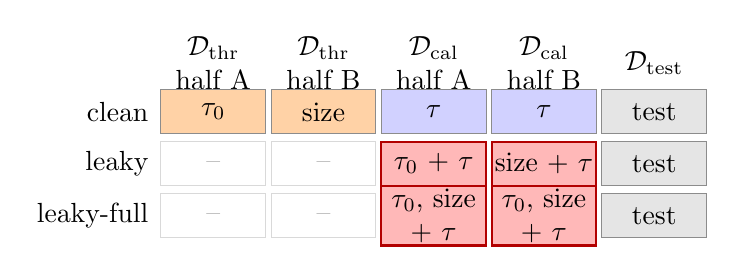
\begin{tikzpicture}[x=1cm, y=1cm,
  box/.style={draw=black!45, minimum width=1.33cm, minimum height=0.56cm,
              inner sep=1pt, align=center},
  srch/.style={box, fill=orange!35},
  fin/.style={box, fill=blue!18},
  reuse/.style={box, fill=red!28, draw=red!70!black, thick},
  tst/.style={box, fill=black!10},
  none/.style={box, draw=black!15, text=black!40}]
\foreach \i/\h in {0/{$\Dthr$\\half A}, 1/{$\Dthr$\\half B},
                   2/{$\Dcal$\\half A}, 3/{$\Dcal$\\half B}, 4/{$\Dtest$}}
  \node[align=center] at (1.55+1.4*\i, 0.62) {\h};
\node[anchor=east] at (0.85, 0)    {clean};
\node[anchor=east] at (0.85, -0.66) {leaky};
\node[anchor=east] at (0.85, -1.32) {leaky-full};
\node[srch]  at (1.55, 0) {$\tau_0$};
\node[srch]  at (2.95, 0) {size};
\node[fin]   at (4.35, 0) {$\tau$};
\node[fin]   at (5.75, 0) {$\tau$};
\node[tst]   at (7.15, 0) {test};
\node[none]  at (1.55, -0.66) {--};
\node[none]  at (2.95, -0.66) {--};
\node[reuse] at (4.35, -0.66) {$\tau_0$ $+$ $\tau$};
\node[reuse] at (5.75, -0.66) {size $+$ $\tau$};
\node[tst]   at (7.15, -0.66) {test};
\node[none]  at (1.55, -1.32) {--};
\node[none]  at (2.95, -1.32) {--};
\node[reuse] at (4.35, -1.32) {$\tau_0$, size\\$+$ $\tau$};
\node[reuse] at (5.75, -1.32) {$\tau_0$, size\\$+$ $\tau$};
\node[tst]   at (7.15, -1.32) {test};
\end{tikzpicture}
\caption{Roles in the hyperparameter search. $\tau_0$: provisional threshold;
size: the mean set size minimized to select a configuration; $\tau$: final
threshold. Red cells feed both the search and the final threshold, which makes
$\tau$ depend on the selection. Mean counts, OmniMedVQA / VQA-RAD: each half
$224$ / $89$ to $90$, $\Dcal$ $448$ / $179$, $\Dtest$ $600$ / $238$.}
\label{fig:roles}
\end{figure}

Under leaky-full, coverage changes by $-0.0100$ for LAC (Holm $p=0.0015$,
Wilcoxon $p=0.0010$) and $-0.0073$ for RAPS ($0.0051$; $0.0016$) on OmniMedVQA,
and set sizes shrink, which is what the search optimizes. APS's change there
and both VQA-RAD changes are not significant (Table~\ref{tab:effects}). A
change is possible only when reuse changes the selected configuration, which
it did on $80\%$ of OmniMedVQA seeds for LAC and RAPS and $15\%$ for APS, and
on $65\%$ and $80\%$ of VQA-RAD seeds for APS and RAPS; that bounds when an
effect can occur, not its size. At $M=1$, with nothing to select, the arms
coincide exactly, and LAC's change grows with the grid it searches
($-0.0046$, $-0.0082$, $-0.0100$ at $M=2,4,6$, each a seeded random subset of
the grid). At matched role sizes the OmniMedVQA LAC and RAPS intervals still
exclude zero, so on that corpus reuse lowers coverage even without the bundle.

\textbf{The binary LAC exception.} At $K=2$, temperature scaling is a common
increasing map of the LAC score: with $d$ the logit gap, $s=\sigma(-d)$ at
$T=1$ and
\begin{equation*}
s_T=\sigma\!\left(\operatorname{logit}(s)/T\right).
\end{equation*}
A strictly increasing map applied to every score preserves calibration ranks,
and with the threshold taken as an unperturbed order statistic $\tau$ moves
with the scores, so the sets do not change. Zeng et al.\
\cite[Prop.~5.1]{zeng2025tuningbias} prove zero tuning bias for temperature
scaling in binary classification. The implementation agrees: across the six
temperatures, probabilities move by up to $0.363$ while every temperature yields
identical sets and an identical selection objective on every seed, so all
three arms pick the first grid entry. The exception is specific to
temperature-only LAC at $K=2$. APS and RAPS, whose scores add a uniform draw
or a rank penalty, are not transformed by one common map, and on OmniMedVQA,
where $K$ is mostly $4$, a temperature changes the sets of up to $25.5\%$ of
items relative to $T=1$.

\subsection{Removing APS's internal randomization}

With $u=1$, APS gives each candidate the cumulative probability through its
rank, so the lower-ranked of two options scores exactly $1$: the scores have an
atom at the top of their range. Dropping $u$ is tempting because it makes sets
reproducible, which recorded seeds already achieve. On VQA-RAD the atom holds
every question whose answer the model ranks second, on average $33.9\%$ of
$\Dcal$, and $51.8\%$ of true-label calibration scores are tied. Only $\alpha$
of the mass may lie above the threshold, so the order statistic lands on the
atom: $\tau=1$ on every re-split, and the inclusive rule admits both options for
every test question, giving coverage $1.0000$ at size $2.0000$. This is an
observed consequence of an atom larger than $\alpha$, not an outcome every
binary classifier must show: a model ranking the true answer second on fewer
than a tenth of questions would avoid it.\rtag{R2.1} On OmniMedVQA $9.5\%$ of true-label
calibration scores are tied without the draw, and deterministic APS spends
$1.276$ extra options per question. Randomization matters here for efficiency;
it is not needed for the lower coverage bound, and it repairs neither
calibration reuse nor clustered sampling.

\section{Beyond marginal coverage}\label{sec:beyond}

\subsection{Subgroups, read against a reference}\label{sec:conditional}

A low worst-group coverage can mean two things: some group really is covered
less often, or small groups give noisy estimates whose minimum is low by
chance. Fig.~\ref{fig:subgroups} shows the first on OmniMedVQA. Marginal
coverage near $0.90$ hides ultrasound at $0.709$ and fundus photography at
$0.984$. Calibrating per modality brings every modality to between $0.892$ and
$0.934$, and pays in set size, most on ultrasound ($2.093$ to $2.918$
options).

\begin{figure}[tb]
\centering
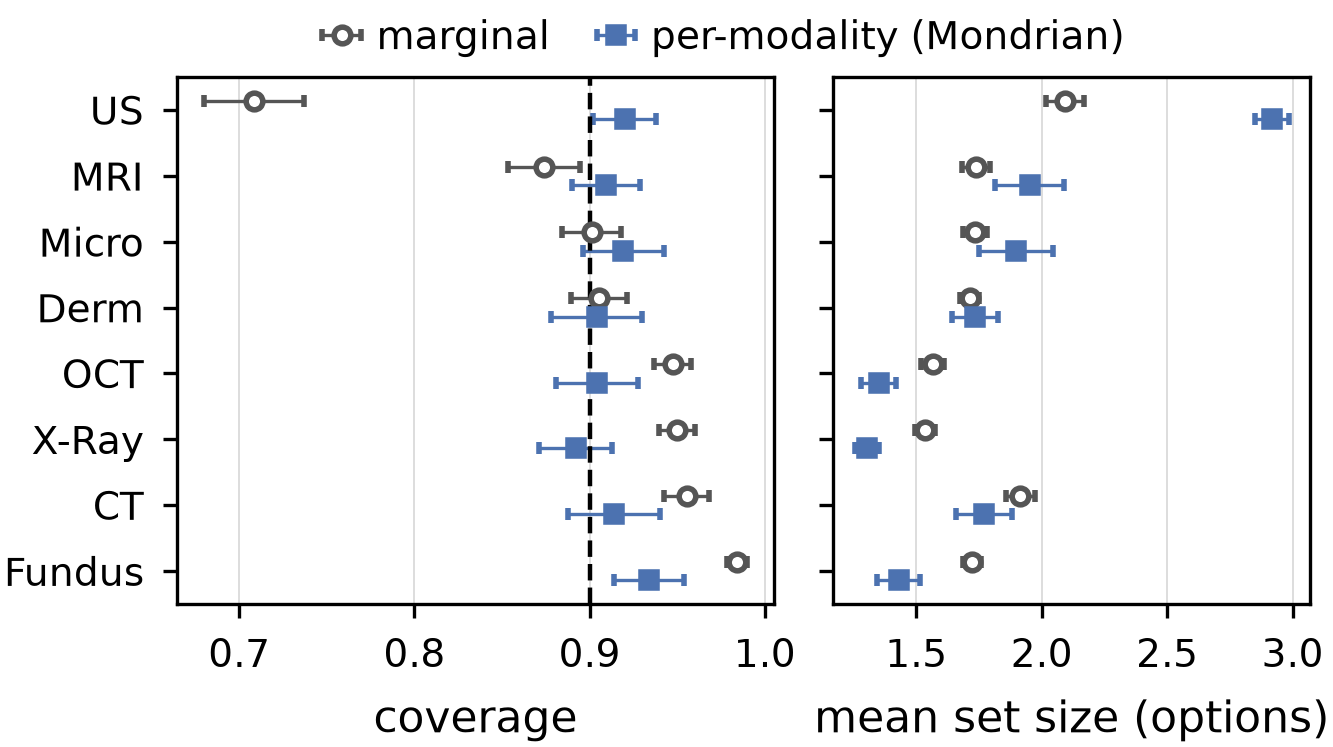
\includegraphics[width=0.95\columnwidth]{B7_subgroups.png}
\caption{OmniMedVQA, LAC at $\alpha=0.10$: per-modality coverage (left) and
mean set size (right) under marginal (open) and per-modality Mondrian
(filled) calibration; means over 20 re-splits with $95\%$ intervals. The
dashed line is the nominal level, not a guarantee for these stratified
splits.}
\label{fig:subgroups}
\end{figure}

To tell the two readings apart when partitions differ in granularity, we
compare each axis with an independent $90\%$-coverage reference at the observed
test-group sizes, simulating each level's coverage as
$\mathrm{Binomial}(n_g,0.9)/n_g$. The reference is descriptive, not the exact
null distribution of this stratified, shared-calibration pipeline. It gives two
summaries (Table~\ref{tab:axes}). \emph{Excess deficit}, the reference's worst
group minus the observed one, speaks to undercoverage. \emph{Excess spread},
the observed $\max-\min$ minus the reference's, speaks to heterogeneity alone,
since coverage of $0.90$ on one group and $1.00$ on another is valid on both.
Letting the threshold vary as well, with all groups of a split sharing one
calibration draw $Q\sim\mathrm{Beta}(k,n+1-k)$ before the binomial step,
changes no excess by more than $0.004$ and leaves the ordering of the axes
unchanged on both corpora.\rtag{R2.5}

\begin{table}[tb]
\caption{Marginal calibration at $\alpha=0.10$ on Qwen2.5-VL-3B, averaged over
the three scores and 20 re-splits. $G$: levels in a test split. Excesses are
relative to an independent $90\%$-coverage reference at the observed level
sizes (positive: worse than the reference).}
\label{tab:axes}
\centering
\footnotesize
\begin{tabular}{lrrrr}
\toprule
Axis & $G$ & Worst & Excess deficit & Excess spread \\
\midrule
\multicolumn{5}{l}{\emph{OmniMedVQA}}\\
modality        & 8   & 0.729 & 0.120    & 0.155 \\
question type   & 5   & 0.808 & 0.048    & 0.096 \\
answer position & 4   & 0.855 & 0.019    & 0.042 \\
option count    & 2.8 & 0.817 & 0.002    & 0.015 \\
source dataset  & 25  & 0.616 & 0.028    & 0.028 \\
\midrule
\multicolumn{5}{l}{\emph{VQA-RAD} (image-disjoint)}\\
organ           & 3   & 0.876 & $-$0.006 & 0.002 \\
answer (yes/no) & 2   & 0.834 & 0.051    & 0.126 \\
\bottomrule
\end{tabular}
\end{table}

The reference reorders the axes. Source dataset has the lowest raw worst-group
coverage, $0.616$, but its excess deficit relative to the reference is
$0.028$, against $0.120$ for modality. With 25 levels, the smallest holding
$3$ test items on average, this comparison is sensitive to the small source
groups. Modality carries the largest excess on both measures, and question
type, an axis this protocol never calibrates on, the second. On VQA-RAD the
released organs give LAC $0.894$ (abdomen) to $0.922$ (chest), close to the
reference at these group sizes ($62$ to $95$ test questions per organ), while
the yes/no split of the correct answer is not (Section~\ref{sec:order}).

Separately from the reference, an approximate test permutes level labels across
a split's test items with the coverage indicators fixed (Pearson $\chi^2$,
$B=2{,}000$, Holm over the five OmniMedVQA axes). It tests association between
level and coverage, not whether every level reaches $0.90$.\rtag{R2.5} It rejects in
$93\%$ of the sixty score-by-re-split runs for modality and $92\%$ for question
type, and in at most $35\%$ for the others. The runs share data, so these
fractions describe stability rather than count independent successes. The test
treats a split's test items as exchangeable, which stratification and ten
images carrying two questions each only approximate; restricting to one
question per image moves no axis's count by more than $4$ of the sixty runs.

\subsection{What Mondrian calibration costs}\label{sec:budget}

Mondrian divides $\Dcal$ among $G$ levels. Subsampling $\Dcal$ on OmniMedVQA
shows that the floor of $9$ is a feasibility condition, not a budget; figures
average the three scores.\rtag{R2.7} At $n_{\mathrm{cal}}=50$ the modalities present in a
subsample hold $6.26$ points on average (a subsample occasionally misses one),
$6.8$ fall below the floor, and Mondrian reports coverage $0.988$ at a mean set
size of $3.71$ options. Above the floor, efficiency still costs data: the
set-size penalty over marginal calibration is $1.921$ options at $6.3$ points
per level, $0.413$ at $12.5$, $0.148$ at $25$ and $0.047$ at the full $56$.
The knee is not fixed. At $\alpha=0.05$ the floor rises to $19$ and the
penalty is still $1.778$ at $12.5$ points per level and $0.223$ at $25$; at
$\alpha=0.20$ (floor $4$) it is $0.228$ and $0.128$. Calibrating on question
type ($G=5$, unbalanced levels) needs about $40$ points per level for a
penalty of $0.138$. In these data useful efficiency required well above the
feasibility floor, and how far above depends on $\alpha$, on the partition and
on the penalty a reader accepts.\rtag{R1.6}

\subsection{Option order}\label{sec:order}

Under marginal calibration, LAC covers $0.947$ of four-option test items whose
answer is printed at A and $0.859$ of those at D. That is observational, since
the items answered at D might be harder, so every item was re-scored under the
three other cyclic rotations of its option list (four of the $24$ orders of a
four-option list), with image, question, option text, model and prompt fixed.
Across the rotations, each item's correct answer appears once behind each
letter. Each presentation's pipeline is tuned on its own $\Dthr$ and calibrated
on its own $\Dcal$, on the same splits, so this compares presentation-specific
tuned and calibrated pipelines. A rotation moves the correct answer and every
distractor together, so the design identifies sensitivity to cyclic
presentation, not a pure answer-letter intervention.

These OmniMedVQA results use the $2{,}745$ items with $K=4$, about $548$ test
items per split.\rtag{C4} Per split we compute coverage in each (letter, rotation) cell.
A letter's profile value averages its four rotation cells with equal weight, an
original index's value averages its four cells, and each profile is then
averaged over re-splits (Fig.~\ref{fig:order}). Summarized by the range of
those means, the original presentation spans $0.088$ for LAC, the letter
profile $0.046$ and the original-index profile $0.047$. Both survive their
averaging, as an item-by-position interaction would, so this is not a claim of
additivity.

\begin{figure}[tb]
\centering
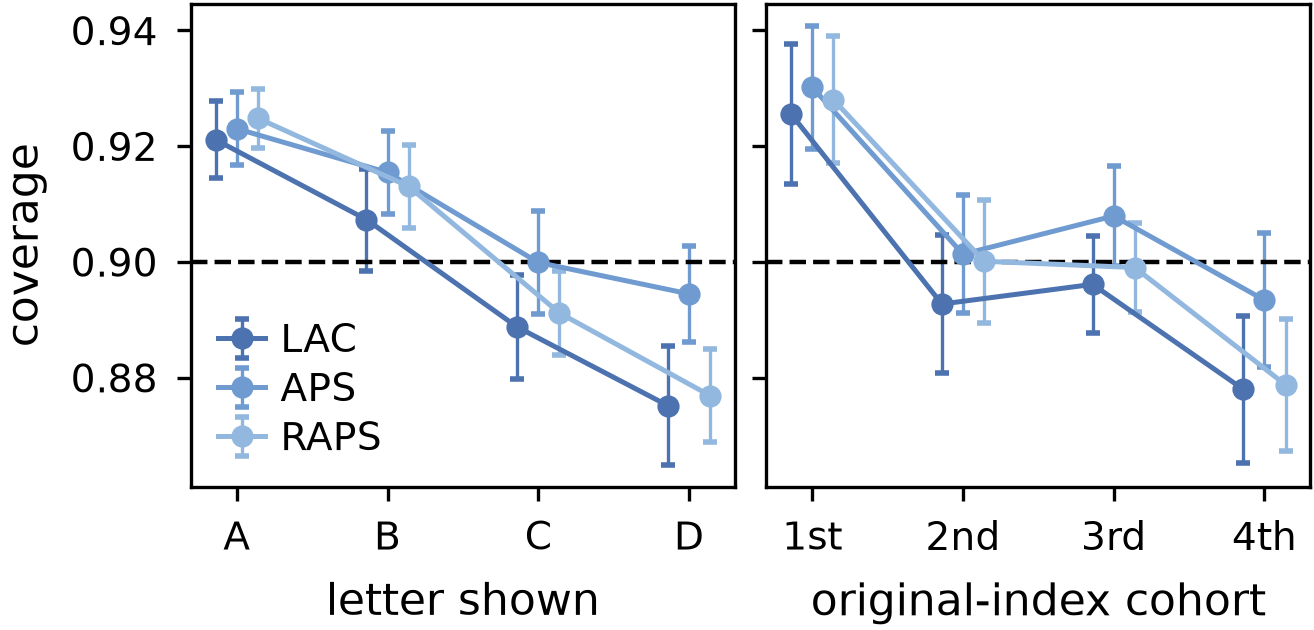
\includegraphics[width=0.95\columnwidth]{B5_order.png}
\caption{OmniMedVQA items with $K=4$, Qwen2.5-VL-3B, marginal calibration,
$\alpha=0.10$; means over 20 re-splits with $95\%$ intervals. Left: coverage
by the letter shown, averaging each letter's four rotation cells. Right: by
the answer's original index, averaging its four letter cells. Dashed: the
nominal level, not a guarantee here.}
\label{fig:order}
\end{figure}

The letter profile is consistent with option-order bias in language-model
multiple choice \cite{zheng2024mcq,pezeshkpour2024order}. The original-index
profile is a cohort difference: items whose answer the corpus placed first are
covered more often, averaged over the four letters. The four cohorts are close
on the composition we measured (total-variation distance from the pooled
distribution at most $0.035$ on modality, $0.029$ on question type and $0.064$
on source), but not in difficulty: rotation-averaged base top-1 runs from
$0.721$ to $0.686$. Recomputing the cohort profile within modality leaves its
spread at $0.0495$, against $0.0475$ overall, and we do not claim that no
unmeasured variable accounts for it. The ensemble averages $\sbase=-\log p$
over the four rotations, a geometric mean of the letter probabilities, and is
tuned and calibrated on the averaged score.\rtag{R2.7} It narrows the range from $0.088$
to $0.059$ for LAC; paired on re-split, the position spread falls for all three
scores (Table~\ref{tab:effects}), and the remainder is not removed.

VQA-RAD, which has no answer-string shortcut, allows a complete design: with
$K=2$, presenting each question in both orders covers every permutation, so
the letter and the correct answer separate exactly. Averaged over both
letters, coverage is $0.991$ for questions whose answer is ``yes'' and $0.833$
for ``no'' (LAC); averaged over both answers, letter A gets $0.916$ and B
$0.908$, with overlapping intervals. For this model on this corpus the order
sensitivity is an answer effect, the model's preference for ``yes'', not a
letter effect, and
averaging the two orders leaves it in place (spread change $-0.004$ [$-0.017$,
$+0.009$], Holm $p=0.729$).\rtag{R1.2}

\section{A second backbone}\label{sec:backbone}
\rtag{R1.1}%
We repeated the analyses of Sections~\ref{sec:protocol} and~\ref{sec:beyond}
on Qwen3-VL-4B with the same items, splits, grids and keyed draws
(Table~\ref{tab:backbone}). It ranks the correct answer first more often and
gives smaller sets at the same coverage.

\begin{table}[tb]
\caption{Both backbones at $\alpha=0.10$, means over 20 re-splits; LAC unless
a row names a score. Worst group: modality or organ. Reuse: leaky-full minus
clean, $^{*}$Holm $p<0.05$ (Section~\ref{sec:setup}). Excess deficit, averaged
over the three scores as in Table~\ref{tab:axes}: modality or yes/no answer.
Order rows average over all presented orders.}
\label{tab:backbone}
\centering
\footnotesize
\setlength{\tabcolsep}{4pt}
\begin{tabular}{lrrrr}
\toprule
 & \multicolumn{2}{c}{OmniMedVQA} & \multicolumn{2}{c}{VQA-RAD} \\
\cmidrule(lr){2-3}\cmidrule(lr){4-5}
 & Qwen2.5 & Qwen3 & Qwen2.5 & Qwen3 \\
\midrule
Top-1 & 0.663 & 0.803 & 0.654 & 0.755 \\
Coverage & 0.903 & 0.907 & 0.907 & 0.904 \\
Size & 1.752 & 1.271 & 1.572 & 1.418 \\
Worst group & 0.709 & 0.805 & 0.868 & 0.880 \\
\midrule
Reuse $\Delta$cov., LAC & $-$0.0100$^{*}$ & $-$0.0040 & 0 & 0 \\
Reuse $\Delta$cov., APS & $-$0.0023 & $-$0.0025 & $-$0.0036 & $-$0.0119$^{*}$ \\
Reuse $\Delta$cov., RAPS & $-$0.0073$^{*}$ & $-$0.0025 & $-$0.0059 & $-$0.0133$^{*}$ \\
APS $u=1$: $\Delta$size & $+$1.276 & $+$0.742 & $+$0.374 & $+$0.548 \\
\midrule
Excess deficit & 0.120 & 0.047 & 0.051 & $-$0.006 \\
Letter-profile range & 0.046 & 0.030 & 0.008 & 0.019 \\
``No'' minus ``yes'' & -- & -- & $-$0.157 & $+$0.057 \\
\bottomrule
\end{tabular}
\end{table}

What follows from the procedures recurs. Deterministic APS again has
$\tau=1$ on every VQA-RAD re-split and returns both options for every question;
its atom now holds $51.9\%$ of $\Dcal$. Calibration reuse leaves binary LAC's
coverage exactly unchanged. Its sets are identical across temperatures except
where floating-point rounding merges near-tied scores at $T=0.25$, which added
options on $2$ of the $20$ re-splits (at most $2.1\%$ of test items) and never
changed coverage.

The magnitudes do not recur. All ten non-zero reuse contrasts lower coverage,
but which survive Holm correction depends on the model: on Qwen3-VL-4B none on
OmniMedVQA, and APS and RAPS on VQA-RAD. Modality still carries the largest
excess deficit on OmniMedVQA, though smaller; the worst modality is now OCT
($0.825$), and ultrasound reaches $0.901$. On VQA-RAD the answer effect
reverses: ``no'' is covered at $0.931$ and ``yes'' at $0.874$, a difference
of $+0.057$ [$+0.037$, $+0.076$], and a letter effect appears (A $0.912$, B
$0.893$). Averaging the two orders removes the letter effect by construction
and so widens the position spread there ($+0.013$, Holm $p=0.013$). On
OmniMedVQA the presentation effects shrink: the original presentation spans
$0.034$ rather than $0.088$, and the order ensemble no longer narrows the
position spread detectably (LAC $-0.006$, Holm $p=0.767$).
Which group is undercovered, and which answer or letter is favoured, are
properties of a model on a corpus, to be measured for each deployment rather
than carried over.

\section{Discussion and limitations}\label{sec:discussion}

\textbf{What should generalize.} Three findings are properties of the
procedures and hold for any model: binary LAC is invariant to temperature
search in exact arithmetic; deterministic APS collapses to all-option sets
whenever its top atom holds more than $\alpha$ of the calibration mass; and
Mondrian levels below $\lceil(1-\alpha)/\alpha\rceil$ return every option. The
first two recurred on the second backbone, the first up to floating-point
ties. The answer-string shortcut is a property of the OmniMedVQA sample, not of
a model. The sizes of the reuse loss, the subgroup gaps and the order profiles
are empirical, and the second backbone changed all three
(Section~\ref{sec:backbone}), although every non-zero reuse effect lowered
coverage.\rtag{R1.4}

\textbf{Implications.} Before crediting a method with a set-size gain, check
what a text-only predictor achieves. Keep score selection separate from final
calibration when using ordinary split conformal without a valid selection
correction \cite{liang2024selection}. Keep APS and RAPS randomized on binary
questions. Choose the Mondrian partition before the score, and budget well
above its floor. Read worst-group coverage against group sizes and alongside
set size, keeping the reference's assumptions in view. Use the same
option-order policy in calibration and prediction, expecting averaging to
reduce letter effects but not answer effects.

\textbf{Split unit.} Against an item-level split on the same seeds, image
disjointness moved none of nine paired VQA-RAD comparisons past Holm
correction (Table~\ref{tab:effects}; all raw $p\ge0.31$) and changed the
leak's size by $+0.0025$ [$-0.0092$, $+0.0141$] for APS and $+0.0012$
[$-0.0122$, $+0.0147$] for RAPS. These are failures to detect a difference,
not evidence of equivalence.\rtag{R1.5} One question per image under an unstratified
uniform split, with the keyed draws above, is a design the theorem does cover;
there, with about $44$ calibration points, pre-fallback coverage is $0.900$,
$0.905$ and $0.903$, and each interval contains the whole band
$[0.900,\,0.922]$.

\textbf{Limitations.} Two backbones from one model family are studied, on two
selected corpora; re-splits of single samples do not measure dataset or
population variability. VQA-RAD holds only 294 images. The four-option order
analysis uses 4 of the 24 permutations and one corpus; only VQA-RAD's binary
case is complete.\rtag{R1.3} Coverage concerns inclusion of the given answer among the
offered options, not the clinical correctness of that answer, and it weighs all
errors equally. We do not rank conformal-training methods
\cite{stutz2022learning,einbinder2022training,shi2025dpsm}; on OmniMedVQA the
shortcut above would make such a ranking hard to interpret.

\textbf{Availability.} Code, item identifiers, split assignments, the VQA-RAD
organ mapping, score caches for both backbones and per-split results are at
\url{https://github.com/ahmedmellit02/3ict}.\rtag{R2.2}

\textbf{Conclusion.} On Qwen2.5-VL-3B, within each corpus the three scores'
mean coverage differed by at most $0.004$ and their set sizes by at most
$0.087$ options, while the calibration-reuse search, removing APS's internal
randomization and calibrating small groups moved coverage or set size by more.
A second backbone kept the procedural effects and changed the empirical ones.
Those effects appear only when the protocol is varied and subgroups are
inspected; marginal coverage and mean set size under one protocol show none of
them.

\bibliographystyle{IEEEtran}
\bibliography{refs}

\end{document}
